\subsection{Sprint 5}

\subsubsection{Introduction}
In this sprint, our focus was on completing the communication between the console and the game using JNI. Backend tasks were assigned for realizing user stories related to establishing communication between the game and the console, while frontend tasks included various implementations for the Pacman game.

\subsubsection{Spikes}

No spikes were conducted in this sprint.

\subsubsection{POCs}

No proofs of concept (POCs) were conducted in this sprint.

\subsubsection{Technical Justification}

During Sprint 0, the team exclusively focused on conducting spikes instead of developing POCs. This decision was based on the following reasons:

\subsubsection{High-Level Architecture (HLArchitecture)}

The architecture followed in this sprint was based on JNI communication between game, bridge, console, and screen.

\begin{itemize}
    \item Architecture: \href{https://github.com/Pending-Name-21/arquitecture/pull/12}{Link to architecture}
    \item C4 DSL Link: \href{https://structurizr.com/dsl}{Visualizer}
\end{itemize}

\newpage


\hypertarget{sos-s3} {
\subsubsection{Scrum of Scrums}\label{Scrum of Scrums} 
At this point, the team was organized to move forward on the console and the Pacman Game.
We mainly updated the UML diagram of the PACMAN game in terms of coalitions, scoring, sprites, movement process and we managed to implement the Game Communication in the Client and Server sockets. Then, in the Daily Lead's we made a conclusion on the pacman UML diagram to move forward on the dependent tasks also on the bridge.jar implementations and finally we finished with a conclusion on what we expect from SOCKETS to use in the library. 
}

\href{https://github.com/Pending-Name-21/arquitecture/pull/11}{Link: UML-Pacman Game - Pull Request on GitHub}.

\href{https://github.com/Pending-Name-21/arquitecture/pull/17}{Link: Game-Comunication - Pull Request on GitHub}.

\begin{figure}
\centering
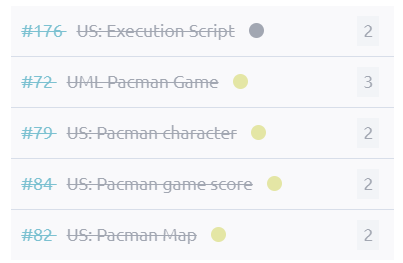
\includegraphics[width=16cm, height=10cm]{./artifacts/src/sprint-5/assets/US-Sprint5.png}
\end{figure}

\hypertarget{burndownchart-s3}{
\subsubsection{Burn Down Chart}\label{Burn Down Chart S3}}
\href{https://tree.taiga.io/project/joseluis-teran-coffeetime/taskboard/sprint-5-3817}{Link: Sprint 5 Board on Taiga}.

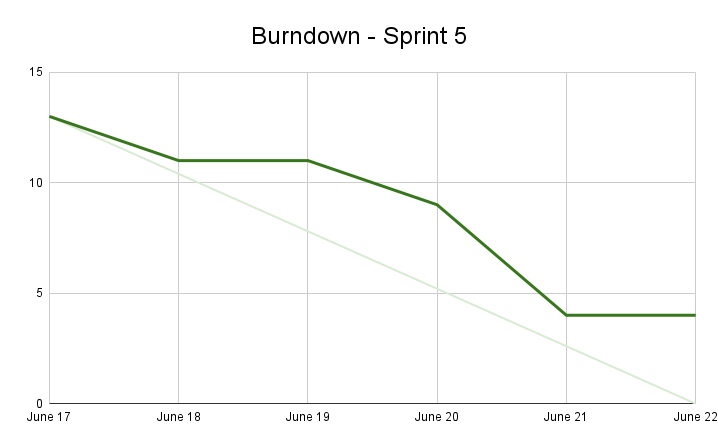
\includegraphics[width=\textwidth]{./artifacts/src/sprint-5/assets/Burndown-Sprint5.png}

\hypertarget{startstopcontinueactionitems-s3}{
\subsubsection{Start-Stop-Continue-Action Items}\label{Start-Stop-Continue-Action Items S6}}
\href{https://miro.com/app/board/uXjVKDO7l8M=/?moveToWidget=3458764590247999187&cot=14}{Link: Start-Stop-Continue-Action Items Sprint 5 on Miro}.

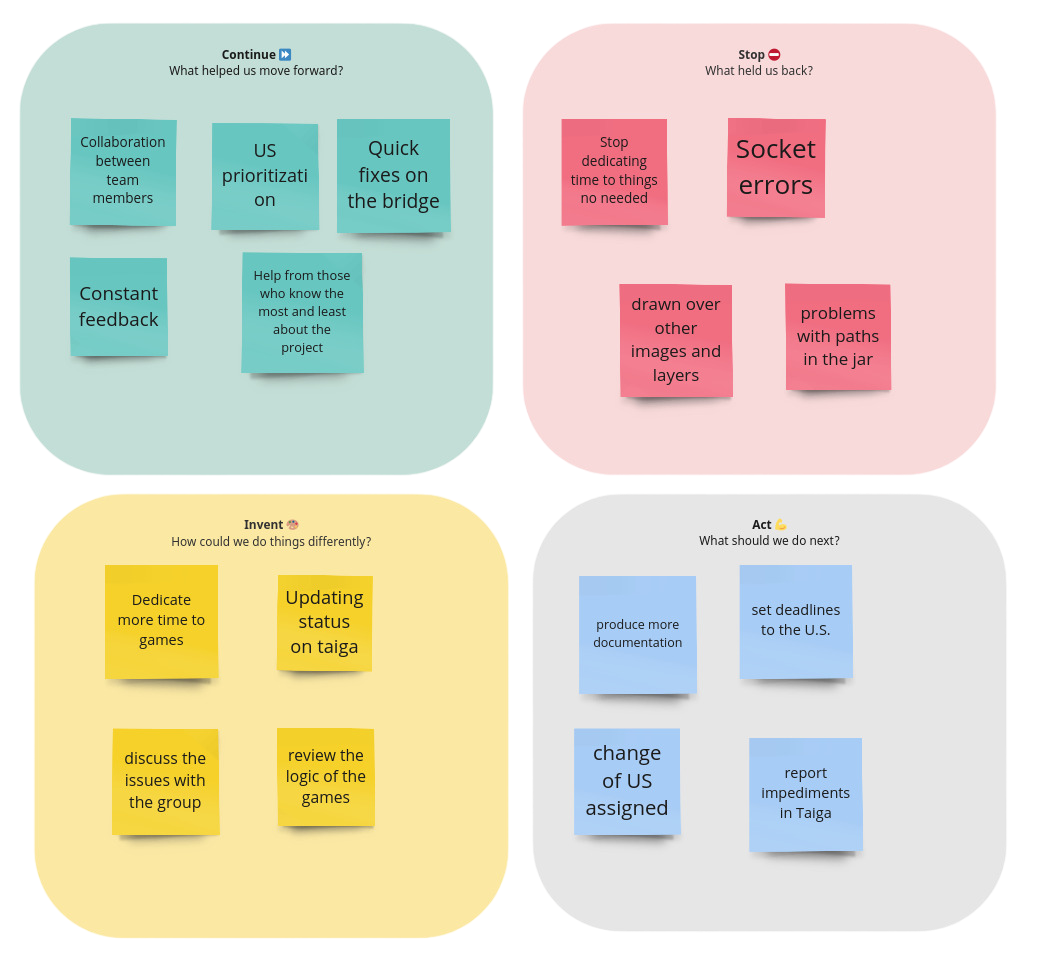
\includegraphics[width=\textwidth]{./artifacts/src/sprint-5/assets/Retrospectives-Sprint5.png}

\documentclass{article}
\usepackage{hyperref}
\usepackage{parskip}

\begin{document}

    \title{Backlog - Sprint 5}
    \author{}
    \date{}
    \maketitle

    \section*{Task Board}
    \href{https://tree.taiga.io/project/joseluis-teran-coffeetime/taskboard/sprint-5-3817}{Sprint 5 Task Board}

    \section*{Completed User Stories}

    \begin{enumerate}
        \item \textbf{Execution Script} \\
        \textit{Assigned to:} Victor Villca \\
        \textit{Status:} Done in Sprint \\
        \textit{Component:} CONSOLE
        \item \textbf{UML Pacman Game} \\
        \textit{Assigned to:} Santiago Concha, Jhael Arce, Victor Villa, Ronaldo Mendoza \\
        \textit{Status:} Done in Sprint \\
        \textit{Component:} PACMAN GAME
        \item \textbf{Pacman Character} \\
        \textit{Assigned to:} Sebastian Barra, Ronaldo Mendoza \\
        \textit{Status:} Done in Sprint \\
        \textit{Component:} PACMAN GAME
        \item \textbf{Pacman Game Score} \\
        \textit{Assigned to:} Victor Villca \\
        \textit{Status:} Done in Sprint \\
        \textit{Component:} PACMAN GAME
        \item \textbf{Pacman Map} \\
        \textit{Assigned to:} Jhael Arce  \\
        \textit{Status:} Done in Sprint \\
        \textit{Component:} PACMAN GAME
    \end{enumerate}

    \section*{Carryover User Stories}

    \begin{enumerate}
        \item \textbf{Colisions on Pacman Game} \\
        \textit{Assigned to:} Victor Villca, Ronaldo Mendoza \\
        \textit{Status:} Carryover \\
        \textit{Component:} PACMAN GAME
        \item \textbf{Game Communication} \\
        \textit{Assigned to:} Josue Prado, Axel Ayala \\
        \textit{Status:} Carryover \\
        \textit{Component:} SCREEN
        \item \textbf{Bridge Screen Communication } \\
        \textit{Assigned to:} Axel Ayala, Santiago Concha, Luiggy Mamani \\
        \textit{Status:} Carryover \\
        \textit{Component:} CONSOLE
    \end{enumerate}

    \section*{Total Points Burned}
    11

\end{document}



\subsubsection{Impediments}
For the impediments we develop a word file:

\href{https://docs.google.com/spreadsheets/d/1S3ndUFktff6ETyNhOyirIFNed71W4ApTLGyjX8xSzUQ/edit?usp=sharing}{impediments}

\subsubsection{Conclusions}

In Sprint 5, our focus was on achieving communication between the game and the console, but the goal was not achieved in this sprint. The most significant progress was seen in the realm of games, specifically in the development of the Pacman Game.

\subsubsection{Action items}

\begin{itemize}
    \item Add priority as tags in the US to make it more visible
\end{itemize}
